In this section, I will explain the setup-by-steo process I took for building
and Active Front End (AFE) in SIMULINK/MATLAB. This involves creating a
three-phase grid, making a three-phase bridge, implementing a line-tophase
voltage conversion function, and developing a three-phase
Phase-Locked-Loop(PLL) for grid sunchronization. I will also cover the park and
clarke transformations, vector magnitude and angle calculation, current
control, and gate time calculation.

\begin{figure}[ht]
    \centering
    \resizebox{\linewidth}{!}{
        \begin{tikzpicture}[auto, node distance=2cm,>=latex']
            % Nodes
            \node [input, name=Vbc] {};
            \node [input, name=Vab, above of=Vbc,node distance=0.7cm] {};
            \node [input, name=Vca, below of=Vbc, node distance=0.7cm] {};
            \node [block, right of=Vbc,node distance=3cm] (phaseline) {Phase-Line Transform};
            \node [block, right of=phaseline,node distance=5cm, minimum height=3cm, minimum width=4cm] (PLL) {Phase Lock Loop};
            \node [block, right of=PLL,yshift=0.5cm,node distance=10cm, minimum height=2.5cm, minimum width=3.5cm] (iclarke) {Inverse Clarke Transform};

            \node [input, name=Ibc, below of=Vbc, node distance=8cm] {};
            \node [input, name=Iab, above of=Ibc,node distance=1cm] {};
            \node [input, name=Ica, below of=Ibc, node distance=1cm] {};
            \node [block, right of=Ibc, node distance=3.5cm, minimum height=3.5cm, minimum width=4.5cm] (park) {Park Transform};

            \node [sum, name=sumID, right of=PLL, yshift=1cm, node distance =5cm]{$+$};
            \node [sum, name=sumIQ, right of=PLL, node distance=6.5cm]{$+$};

            \node [block, name=svm, right of=PLL, node distance=15.5cm, minimum height=3.5cm, minimum width=4.5cm]{Space Vector Modulation};

            \node [block, name=piID, right of=park, node distance=6.5cm, yshift=1cm]{PI\\Controller};
            \node [block, name=piIQ, right of=park, node distance=6.5cm, yshift=-1cm]{PI\\Controller};

            \node [sum, name=setIQ, left of=piID, node distance=2.5cm]{};
            \node [sum, name=setID, left of=piIQ, node distance=2.5cm]{};

            \node [input, name=Id, below of=setID, node distance=2cm]{};
            \node [input, name=Iq, above of=setIQ, node distance=2cm]{};

            \node [output, name=gb, right of=svm, node distance=4cm]{};
            \node [output, name=ga, above of=gb, node distance=1cm]{};
            \node [output, name=gc, below of=gb, node distance=1cm]{};

            % Connections
            \draw[->] (Vab) node[above]{$V_{ab}$} -- ([yshift=0.7cm]phaseline.west);
            \draw[->] (Vbc) node[above]{$V_{bc}$} -- (phaseline.west);
            \draw[->] (Vca) node[above]{$V_{ca}$} -- ([yshift=-0.7cm]phaseline.west);

            \draw[->] ([yshift=0.7cm]phaseline.east) node[above right]{$V_{a}$} -- ([yshift=0.7cm]PLL.west);
            \draw[->] (phaseline.east) node[above right]{$V_{b}$} -- (PLL.west);
            \draw[->] ([yshift=-0.7cm]phaseline.east) node[above right]{$V_{c}$} -- ([yshift=-0.7cm]PLL.west);

            \draw[->] (Iab) node[above]{$I_{a}$} -- ([yshift=1cm]park.west);
            \draw[->] (Ibc) node[above]{$I_{b}$} -- (park.west);
            \draw[->] (Ica) node[above]{$I_{c}$} -- ([yshift=-1cm]park.west);

            \draw[->] ([yshift=1cm]PLL.east) node[above right]{$V_d$} -- (sumID.west);
            \draw[->] (PLL.east) node[above right]{$V_q$} -- (sumIQ.west);
            \draw[->] (sumID.east) node[above right]{$V_d^*$} -- ([yshift =0.5cm]iclarke.west);
            \draw[->] (sumIQ.east) node[above right]{$V_q^*$} -- ([yshift =-0.5cm]iclarke.west);

            \draw[->] ([yshift=0.5cm]iclarke.east) node[above right]{$V_\alpha^*$} -- ([yshift=1cm]svm.west);
            \draw[->] ([yshift=-0.5cm]iclarke.east) node[above right]{$V_\beta^*$} -- (svm.west);
            \draw[->] ([yshift=-1cm]PLL.east) node[above right]{$\theta$} -- ([yshift=-1cm]svm.west);

            \draw[->] (piID.east) node[above right]{$\Delta V_d$} -|(sumID.south);
            \draw[->] (piIQ.east) node[above right]{$\Delta V_q$} -|(sumIQ.south);

            \draw[->] (setIQ.east) -- (piID.west);
            \draw[->] (setID.east) -- (piIQ.west);

            \draw[->] (Iq) node[right]{$I_q^*$} -- (setIQ.north);
            \draw[->] (Id) node[right]{$I_d^*$} -- (setID.south);

            \draw[->] ([yshift=1cm]park.east) node[above right]{$I_q$} -- (setIQ.west);
            \draw[->] ([yshift=-1cm]park.east) node[above right]{$I_d$} -- (setID.west);

            \draw[->] ([yshift=-1cm,xshift=2cm]PLL.east)--([yshift=-3.5cm,xshift=2cm]PLL.east)-|(park.north);

            \draw[->] ([yshift=1cm]svm.east) node[above right]{$V_a^*$} -- (ga);
            \draw[->] (svm.east) node[above right]{$V_b^*$} -- (gb);
            \draw[->] ([yshift=-1cm]svm.east) node[above right]{$V_c^*$} -- (gc);
        \end{tikzpicture}
    }
    \caption{Active Front End Converter}
    \label{fig:FEC}
\end{figure}

\subsection{Three-phase Grid}
\begin{figure}[h]
    \centering
    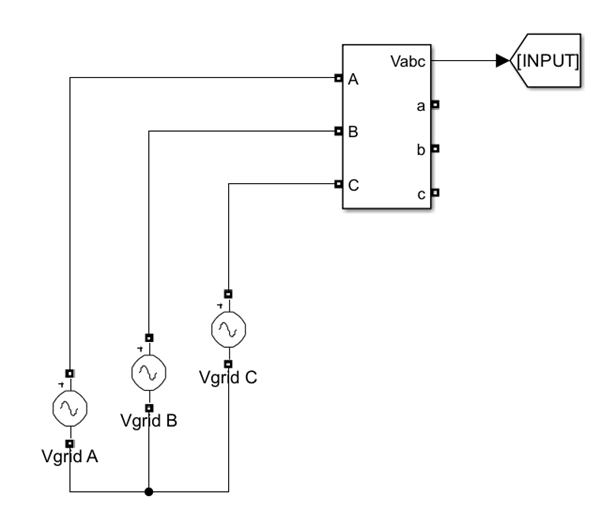
\includegraphics[width=0.5\textwidth]{grid.png}
    \caption{Three Phase Grid in SIMULINK}
    \label{fig:Grid}
\end{figure}
To begin, I created a three-phase grid using SIMULINK's AC source block. This
grid represents the primary input power supply to the system. By connecting
three AC source blocks in a star configuration, I established a three-phase AC
source. Additionally, I added a three-phase VI measurement block to accurately
measure the grid voltage, which I labeled as $INPUT$ to maintain clarity within
the simulation environment.

\subsection{Three-Phase Bridge}
\begin{figure}[h]
    \centering
    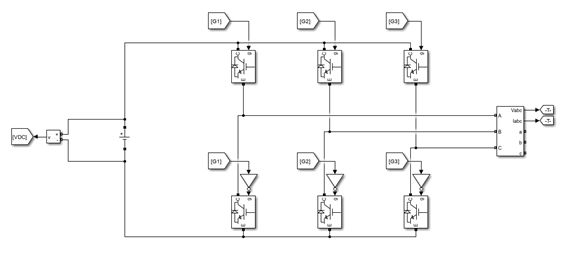
\includegraphics[width=0.8\textwidth]{bridge.png}
    \caption{Front End Conveerter IGBT Bridge}
    \label{fig:Bridge}
\end{figure}
To proceed, I constructed a three-phase bridge using Insulated Gate Bipolar
Transistors (IGBTs) within SIMULINK. Each IGBT gate was labeled as G1, G2, and
G3.\\

To power the bridge, a DC voltage source was added. This source provided the
necessary voltage to drive the IGBTs and maintain stable operation of the
bridge circuit. A voltage measurement block, labeled as VDC, was included to
monitor the DC voltage across the bridge. This measurement block enabled
real-time monitoring and adjustment of the DC voltage level during
simulation.\\

For monitoring the output of the bridge, a three-phase VI measurement block was
connected to the bridge's output terminals. This block facilitated the
measurement and monitoring of both the output voltage (labeled as Vout) and
current (labeled as Iout). These measurements were crucial for the control
system to generate the necessary gate pulses for the IGBTs.

\subsection{Line-To-Phase Voltage conversion}
To apply control algorithms, I needed to convert the measured phase voltages to
line voltages. This involves defining a transformation matrix and implementing
it in a MATLAB function block.

\begin{lstlisting}[style=MATLAB, caption={Phase to Line voltage transformation function}, label={lst:matlab}]
    function [Va, Vb, Vc] = lineToPhase(Vab, Vbc, Vca)
    % Accepts three variables Vab, Vbc, and Vca representing phase voltages
    
    % Combine inputs into a matrix
    V = [Vab, Vbc, Vca];
    
    % Transformation matrix
    T = [2/3, 1/3, 0;
         -1/3, -1/3, 0;
         -1/3, -2/3, 0];
    
    % Calculate phase voltages
    PhaseVoltages = T * V;
    
    % Extract individual phase voltages
    Va = PhaseVoltages(1);
    Vb = PhaseVoltages(2);
    Vc = PhaseVoltages(3);
    end
\end{lstlisting}

\begin{figure}[h]
    \centering
    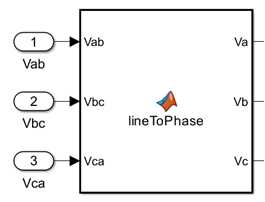
\includegraphics[width=0.5\textwidth]{linefunction.png}
    \caption{Phase-Line Voltage Conversion function}
    \label{fig:phase}
\end{figure}

\subsection{Three-Phase Phase-Locked Loop (PLL)}
The PLL is crucial for accurately measuring the phase and frequency of the grid
voltage, which is essential for generating constant voltages via the Park
transformation. These voltages are subsequently used for current control within
the Active Front End (AFE).\\

I implemented a MATLAB function block in SIMULINK to perform PLL operations.
This function takes line voltages as inputs and outputs park voltages along
with the phase angle ($\theta$).\\

\begin{lstlisting}[style=MATLAB, caption={Three-Phase Phase-Locked Loop}, label={lst:matlab}]
    function [Vd, Vq, theta_o] = PLL(Va, Vb, Vc)
    % Proportional and Integral Controller Parameters
    kp = 28.935; % Proportional gain
    ki = 173610; % Integral gain
    
    % Sampling Time
    dt = 1e-4; % Time step
    
    % Persistent Variables Initialization
    persistent theta; % Phase angle
    if isempty(theta)
        theta = 0;
    end
    
    persistent pid_i; % Integral term of PID controller
    if isempty(pid_i)
        pid_i = 0;
    end
    
    % Park Transformation Matrix
    phi = (2*pi)/3;
    T = [cos(theta), cos(theta - phi), cos(theta + phi);
         sin(theta), sin(theta - phi), sin(theta + phi)] * (2/3);
     
    % Input Vector
    Vabc = [Va; Vb; Vc];
    
    % Park Transformation
    ParkVoltages = T * Vabc;
    Vd = ParkVoltages(1);
    Vq = ParkVoltages(2);
    
    % Error Calculation
    error = Vq;
    
    % PID Controller
    pid_p = kp * error; % Proportional term
    pid_i = pid_i + ki * error * dt; % Integral term
    pid = pid_p + pid_i; % Total PID output
    
    % Frequency Calculation
    omega = 2*pi*50 + pid;
    
    % Phase Angle Integration
    theta = theta + (omega * dt);
    
    % Roll back to zero if theta exceeds 2*pi
    if theta > 2*pi
        theta = 0;
    end
    
    % Output the phase angle
    theta_o = theta;
end
\end{lstlisting}

\subsection{$DQ0-\alpha\beta0$ Transformation}
The newly calculated voltages \( V_d^* \) and \( V_q^* \) are derived from the
output of the current PI loops. These voltages represent the transformed
components in the stationary reference frame after applying the Inverse Clarke
transform, which converts them from the rotating reference frame. This
transformation is crucial for subsequent calculations, such as determining the
timings required for space vector modulation.\\

In the provided MATLAB function block shown in Listing \ref{lst:iclarke}, the
\( DQ \)-\( \alpha\beta \) transformation is implemented using matrix
operations.\\

\begin{lstlisting}[style=MATLAB, caption={Three-Phase Phase-Locked Loop}, label={lst:iclarke}]
    function [alpha, beta] = DQ_AlphaBeta(D, Q, angle)
    % Transformation Matrix
    T = [cos(angle), -sin(angle);
         sin(angle), cos(angle)];
     
    % Input Vector
    DQ = [D; Q];
    
    % AlphaBeta Transformation
    AlphaBeta = T * DQ;
    alpha = AlphaBeta(1);
    beta = AlphaBeta(2);
end
\end{lstlisting}

\subsection{Reference Signal Generator}

\begin{figure}[h]
    \centering
    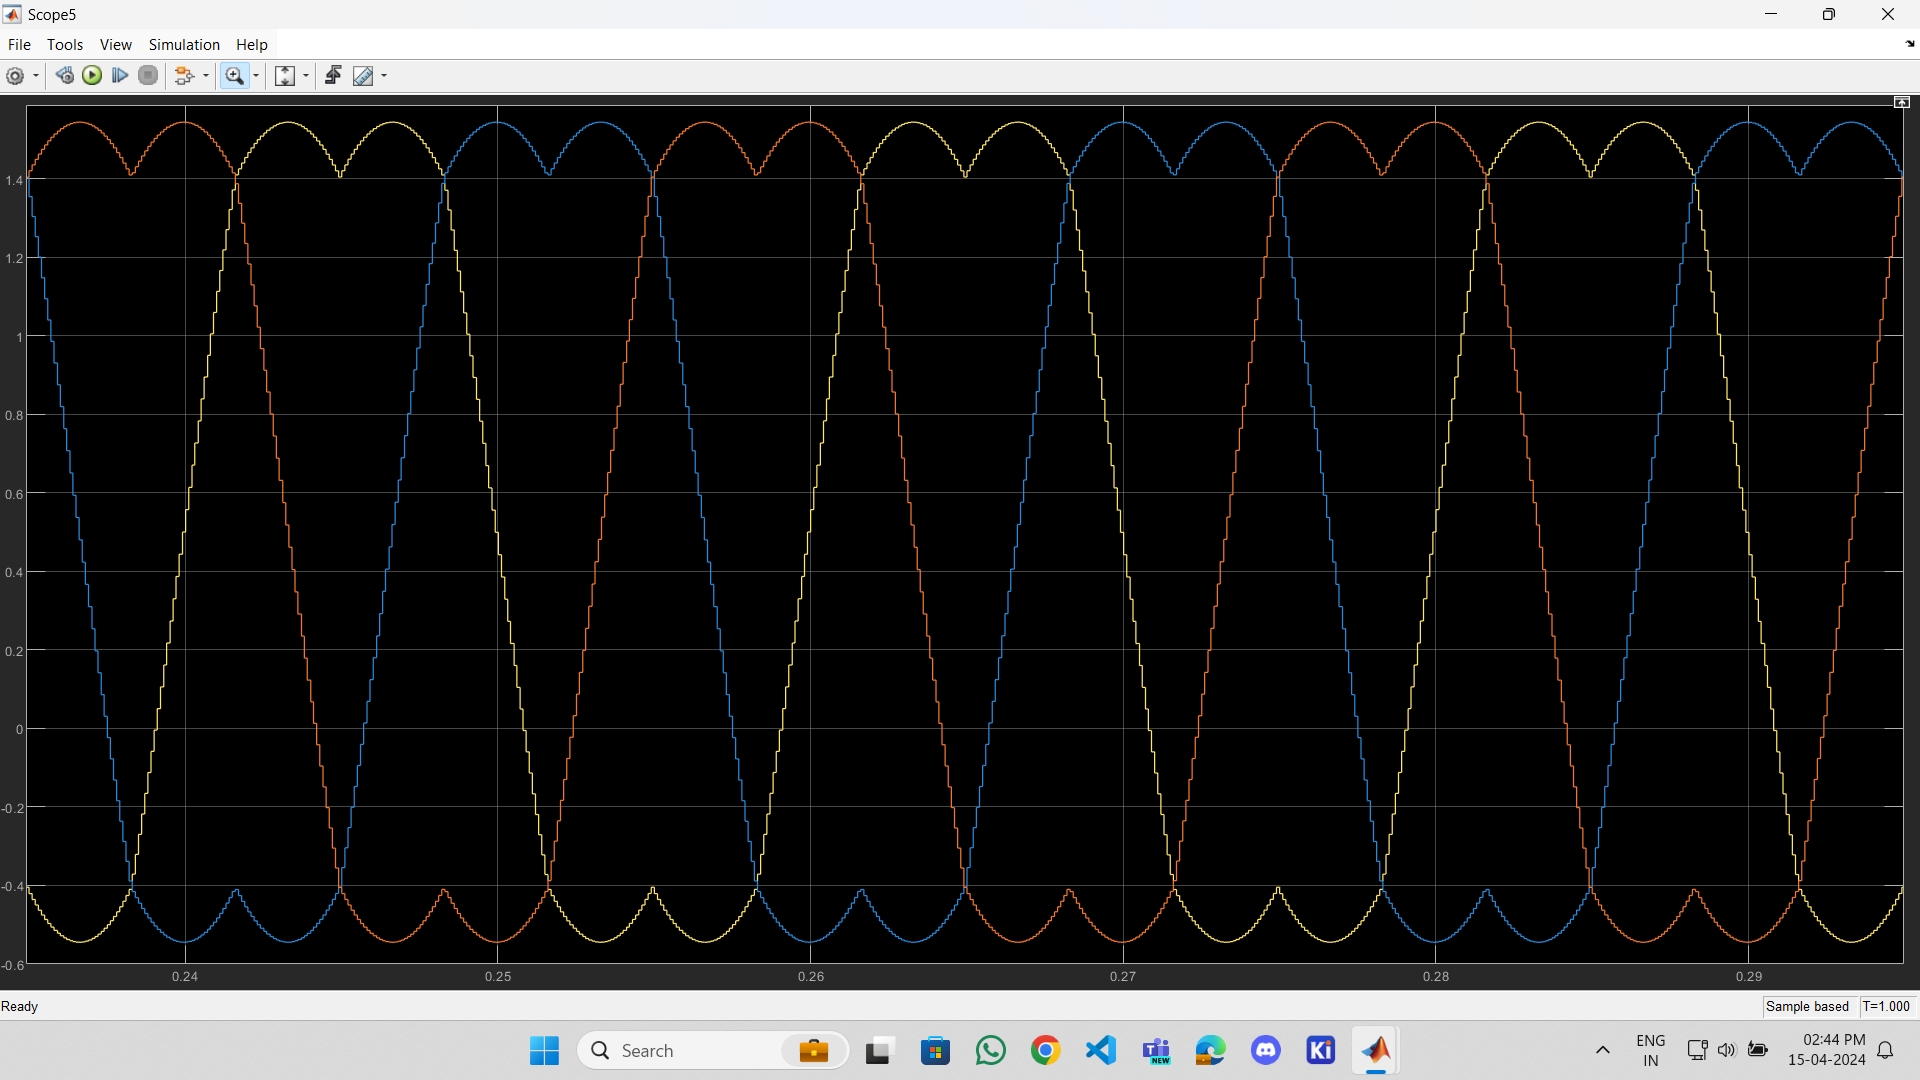
\includegraphics[width=1\textwidth]{matlabsvpwm.png}
    \caption{Space Vector Modulation }
    \label{fig:spaceyfinal}
\end{figure}
The Reference Signal Generator is responsible for generating the reference
signals required for controlling the active front end. These signals,
represented in the \( \alpha\beta0 \) frame, are used to create space vector
modulated signals for the three phases. These modulated signals are compared
with a triangle wave to generate the PWM signal for controlling the IGBT.

\subsubsection{Polar Voltage Conversion}
The new Clarke voltages obtained from the inverse Clarke transform function are
converted to polar voltages. The magnitude of the vector is calculated using
the Pythagorean theorem:
\begin{equation*}
    V = \sqrt{\alpha^2 + \beta^2}
\end{equation*}

To calculate the vector angle, the `atan2` function is used because it provides
angles within the range of \( -2\pi \) to \( 2\pi \):
\begin{equation*}
    \theta = \text{atan2}(\alpha,\beta)
\end{equation*}

\begin{lstlisting}[style=MATLAB, caption={Polar Vector Calculation}, label={lst:polar}]
    V = sqrt(alpha^2 + beta^2);
    
    theta = atan2(alpha,beta);
    if theta < 0 
        theta = theta + 2*pi;
    end
\end{lstlisting}

\subsubsection{Vector Time Calculation}
Using the polar voltages derived from the inverse Clarke transform, the active
vector timings and gate pulse timings are calculated using space vector
modulation. The converter switches through vector states such that only one leg
of the converter changes state at any given time.

\begin{lstlisting}[style=MATLAB, caption={Vector Time Calculation}, label={lst:vector_time}]
    sector = ceil(6 * mod(\theta, 2\pi) / (2\pi));

    TA = V * sin(sector*pi/3 - \theta);
    TB = V * sin(-(sector-1)*pi/3 + \theta);
    T0 = 1 - TA - TB;

    switch sector 
        case 1 
            s1 = TA + TB + T0/2; 
            s2 = TB + T0/2; 
            s3 = T0/2; 
        case 2 
            s1 = TA + T0/2; 
            s2 = TA + TB + T0/2; 
            s3 = T0/2; 
        case 3 
            s1 = T0/2; 
            s2 = TA + TB + T0/2; 
            s3 = TB + T0/2; 
        case 4 
            s1 = T0/2; 
            s2 = TA + T0/2; 
            s3 = TA + TB + T0/2; 
        case 5 
            s1 = TB + T0/2; 
            s2 = T0/2; 
            s3 = TA + TB + T0/2; 
        otherwise 
            s1 = TA + TB + T0/2; 
            s2 = T0/2; 
            s3 = TB + T0/2; 
    end
\end{lstlisting}

In Listing \ref{lst:vector_time}, the MATLAB function calculates the Switch
timings \( s1 \), \( s2 \), and \( s3 \) based on the sector in which the angle
\( \theta \) falls. These timings are crucial for generating the gate pulse
signals that control the IGBTs in the active front end, ensuring proper
modulation of the output voltage.

\subsection{Current Controller}

\begin{figure}[h]
    \centering
    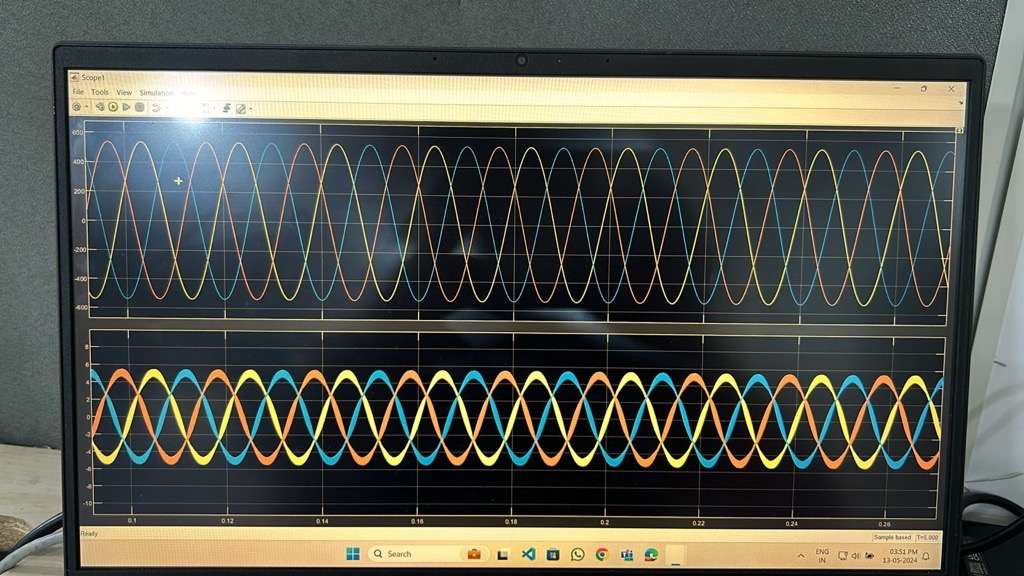
\includegraphics[width=1\textwidth]{Final.jpg}
    \caption{Closed Loop Simulation}
    \label{fig:final}
\end{figure}

The Current Controller plays a crucial role in regulating the output voltage to
achieve precise current control. It operates by converting the line currents
into the DQ-frame of reference and then feeding these components into a PI
controller.

\subsubsection{Park Transformation Function}

The Park transformation function, as shown in Listing \ref{lst:parktransform},
converts the three-phase currents \( I_a, I_b, I_c \) into the DQ-frame of
reference. This transformation aligns the current components \( I_d \) (direct
axis) and \( I_q \) (quadrature axis) with the rotating reference frame, which
is defined by the angle \( \theta \) obtained from the voltage Phase-Locked
Loop (PLL). This alignment ensures that the current remains in phase with the
voltage, thereby achieving a unity power factor.

\begin{lstlisting}[style=MATLAB, caption={Park Transformation}, label={lst:parktransform}]
function [iq, id] = current_transform(ia, ib, ic, theta)
    % Input Vector
    Iabc = [ia; ib; ic];

    % Transformation Matrix
    T = (2/3) * [cos(theta), cos(theta - (2*pi)/3), cos(theta + (2*pi)/3);
                sin(theta), sin(theta - (2*pi)/3), sin(theta + (2*pi)/3)];

    % Park Transformation
    Idq = T * Iabc;
    id = Idq(1);
    iq = Idq(2);
end
\end{lstlisting}

\subsubsection{PI Controller}

The PI Controller, depicted in Listing \ref{lst:picontroller}, operates based
on the \( I_q \) component derived from the Park transformation. It adjusts the
demand \( V_d \) based on the error between the desired \( I_q \) setpoint and
the actual \( I_q \) current. This control loop maintains precise current
levels.\\

\begin{lstlisting}[style=MATLAB, caption={PI Controller}, label={lst:picontroller}]
function Vd_demand = PI_Controller_q(iq, iq_set)
    dt = 1e-4;
    
    persistent pid_i; % Integral term of PID controller
    if isempty(pid_i)
        pid_i = 0;
    end
    
    % Proportional and Integral Controller Parameters
    kp = 47.25; % Proportional gain
    ki = 17010; % Integral gain
    
    % Error Calculation
    error = iq_set - iq;
    
    % PID Controller
    pid_p = kp * error; % Proportional term
    pid_i = pid_i + ki * error * dt; % Integral term
    pid = pid_p + pid_i; % Total PID output
    
    Vd_demand = pid;
end
\end{lstlisting}

These components work in tandem to ensure that the current is precisely
controlled, aligning with the voltage phase to maintain optimal performance and
power efficiency in the active front end.
